\subsection{$\LINAEXPTIME$ MC algorithm for $\AAbarBBbarEbar$}\label{sec:UpperBound}

In this section, taking advantage of the  exponential small-model property proved previously, we design a MC algorithm for $\AAbarBBbarEbar$ formulas with regular expressions belonging to the complexity class $\LINAEXPTIME$.
We recall that  $\LINAEXPTIME$ is the class of problems solvable by  singly exponential-time bounded alternating Turing machines (ATMs, for short) performing at most a polynomial-bounded number of alternations. More formally, an ATM $\M$ (we refer to~\cite{CKS81} for standard syntax and semantics of ATMs)  is \emph{singly exponential-time bounded} if there exists an integer constant $c\geq 1$ such that, for each input $\alpha$, any computation starting on  $\alpha$
 %, no matter what are the universal and existential choices, $\M$ 
 halts after at most $2^{|\alpha|^{c}}$ steps. The ATM $\M$ makes a \emph{polynomial-bounded number of alternations} if there exists an integer constant $c'\geq 1$ such that, for all inputs $\alpha$ and computations $\pi$ starting from $\alpha$, the number of alternations of existential and universal configurations along $\pi$ is at most $|\alpha|^{c'}$.

In the sequel, we restrict ourselves w.l.o.g.\ to
$\AAbarBBbarEbar$  formulas in
\emph{negation normal form} (\nnf). 
 For $\varphi$ in \nnf, the \emph{dual}
 of  $\varphi$, denoted as $\widetilde{\varphi}$, is defined as  the \nnf\ of $\neg\varphi$.
%
The complexity measure of an $\AAbarBBbarEbar$ formula $\varphi$ that we will consider is
the standard  \emph{alternation depth}, denoted by $\AltN(\varphi)$, between the existential $\hsX$  and universal
modalities $\hsXu$ (and vice versa) occurring in the \nnf{} of $\varphi$, \emph{for $X\in \{\overline{B},\overline{E}\}$}. Note that the definition does not consider the modalities associated with the Allen's relations in $\{A,\overline{A},B\}$. 
Moreover, let $\FMC$ be the set of pairs $(\Ku,\varphi)$ consisting of a finite Kripke structure $\Ku$ and an $\AAbarBBbarEbar$ formula $\varphi$ such that $\Ku\models\varphi$ (i.e., $\Ku$ is a model of $\varphi$). 

The following theorem states the complexity upper bound of MC for $\AAbarBBbarEbar$ formulas with regular expressions.


% For technical convenience, we can also assume that the   ATM $\M$ contains a set of \emph{deterministic} states leading to deterministic configurations which have at most one successor.
% The main result of this section is given by the following theorem, which is crucially based on Theorem~\ref{theorem:singleExpTrackModel}.
%In fact, by using Theorem~\ref{theorem:singleExpTrackModel}, it is a relatively simple task to construct a singly exponential-time bounded ATM accepting $\FMC$ with a number of alternations linear in the size of the given input $\varphi$. However, enforcing the number of alternations to match the weak alternation depth $\Upsilon_w(\varphi)$ makes the construction a little more complicated.

\begin{theorem}\label{Theorem:UpperBoundAAbrBBarEbar} One can construct a singly exponential-time bounded ATM accepting $\FMC$ whose number of alternations on an input $(\Ku,\varphi)$ is at most $\AltN(\varphi)+2$.
\end{theorem}

To prove the assertion  of Theorem~\ref{Theorem:UpperBoundAAbrBBarEbar}, we define a procedure in the remaining part of the section. Such a procedure can be easily translated into an ATM (the translation is omitted).

We start with some auxiliary notation. Let us fix a finite Kripke structure $\Ku$ with set of states $\States$ and an $\AAbarBBbarEbar$ formula $\varphi$ in \nnf.
Let $h=\nestb(\varphi)$, and
$\SPEC$ be the set of regular expressions occurring in $\varphi$.
%
A \emph{certificate} of $(\Ku,\varphi)$ is a trace $\rho$ of $\Ku$ whose length is less than $(|S|\cdot 2^{(2|\SPEC|)^2})^{h+2}$ (the bound for the exponential small-model property of Theorem~\ref{theorem:singleExpTrackModelRegex}).
%Fix a certificate $\rho$.
A \emph{$\overline{B}$-witness} (resp., \emph{$\overline{E}$-witness}) of a certificate $\rho$ for $(\Ku,\varphi)$ is a certificate $\rho'$ of  $(\Ku,\varphi)$ such that $\rho'$ is $h$-prefix bisimilar to a trace having the form $\rho\star \rho''$ (resp., $\rho''\star \rho$) for some
\emph{certificate} $\rho''$ of $(\Ku,\varphi)$ with $|\rho''|>1$. Finally, by $\SD(\varphi)$ we denote the set consisting of the subformulas $\psi$ of $\varphi$ and  the \emph{duals} $\widetilde{\psi}$.

The results stated in Section~\ref{sec:AAbarBBbarEbarTrackProperty} are used to prove the properties of certificates, which are listed in the following Proposition~\ref{prop:EbarBbarWitness}, and then exploited in the MC algorithm.
%
\begin{proposition}\label{prop:EbarBbarWitness} Let $\Ku$ be a finite Kripke structure,  $\varphi$ be an $\AAbarBBbarEbar$ formula  in \nnf, and $\rho$ be a certificate for $(\Ku,\varphi)$. The next properties hold:
\begin{enumerate}
  \item for each $\hsX\psi\in\SD(\varphi)$, with $X\in \{\overline{B}, \overline{E}\}$, it holds $\Ku,\rho\models \hsX\psi$ if and only if there exists an $X$-witness $\rho'$ of $\rho$
  for $(\Ku,\varphi)$ such that $\Ku,\rho'\models \psi$;
  \item for each trace having the form $\rho\star\rho'$ (resp., $\rho'\star\rho$) such that $\rho'$ is a certificate for $(\Ku,\varphi)$, one can construct in time singly exponential in the size of $(\Ku,\varphi)$,
  a certificate $\rho''$ which is $h$-prefix bisimilar to $\rho\star\rho'$ (resp., $\rho'\star\rho$), with $h=\nestb(\varphi)$.
\end{enumerate}
\end{proposition}
\begin{proof} 
$(1.)$ Let $\hsX\psi\in\SD(\varphi)$  with $X\in \{\overline{B}, \overline{E}\}$, $h=\nestb(\varphi)$, and $\rho$ be a certificate for $(\Ku,\varphi)$. Let us assume that $X= \overline{E}$  (the  case for $X= \overline{B}$ is similar). 

First we assume that there exists an  $\overline{E}$-witness $\rho'$ of $\rho$ for $(\Ku,\varphi)$ such that $\Ku,\rho'\models \psi$. Hence $\rho'$ is $h$-prefix bisimilar to a trace having the form $\rho''\star \rho$, with $|\rho''|>1$. Since $\hsEt\psi\in\SD(\varphi)$, it holds that
$\nestb(\hsEt\psi)\leq h$. By Proposition~\ref{prop:fulfillmentPreservingPrefix} we have that  $\Ku, \rho''\star \rho \models \psi$ and, then, $\Ku,\rho\models \hsEt\psi$.

To prove the converse implication, we assume that $\Ku,\rho\models \hsEt\psi$. Then, there exists a trace having the form $\rho''\star \rho$ with $|\rho''|>1$ such that
$\Ku,\rho''\star\rho\models \psi$. By Theorem~\ref{theorem:singleExpTrackModelRegex} there exists a certificate $\nu$ for $(\Ku,\varphi)$ which is $h$-prefix bisimilar
to $\rho''$. By Proposition~\ref{prop:invarianceLeftRightPrefix}, $\nu\star \rho$ is $h$-prefix bisimilar to  $\rho''\star\rho$. By applying Proposition~\ref{prop:fulfillmentPreservingPrefix} we deduce that $\Ku,\nu\star\rho\models \psi$. By applying again Theorem~\ref{theorem:singleExpTrackModelRegex}, there exists
a certificate $\rho'$ for $(\Ku,\varphi)$ which is $h$-prefix bisimilar to  $\nu\star \rho$ such that $\Ku,\rho'\models \psi$. Thus, since $\rho'$ is an
$\overline{E}$-witness of $\rho$ for $(\Ku,\varphi)$, $(1.)$ follows. 

$(2.)$ From the trace $\rho\star\rho'$ (resp., $\rho'\star\rho$), where both $\rho$ and $\rho'$ are certificates for $(\Ku,\varphi)$, we first compute the $h$-prefix sampling of $\rho\star\rho'$ (resp., $\rho'\star\rho$), where $h=\nestb(\varphi)$. Then, proceeding as in the proof of Theorem~\ref{theorem:singleExpTrackModelRegex}, we extract from
$\rho\star\rho'$ (resp., $\rho'\star\rho$) a trace which is $h$-prefix bisimilar to $\rho\star\rho'$ (resp., $\rho'\star\rho$). Since $|\rho|$ and $|\rho'|$ are singly exponential in the sizes of $(\Ku,\varphi)$, $(2.)$ follows.
\end{proof}


Let $\AAbar(\varphi)$ be the set of formulas in $\SD(\varphi)$ having the form $\hsX\psi'$ or $\hsXu\psi'$, with $X\in \{A,\overline{A}\}$.
An $\AAbar$-labeling $\GLab$ for $(\Ku,\varphi)$ is a mapping associating with each state $s$ of $\Ku$ a maximally consistent set of subformulas of $\AAbar(\varphi)$. More precisely, for all $s \in \States$, $\GLab(s)$ is such that for all $\psi,\widetilde{\psi}\in \AAbar(\varphi)$, $\GLab(s)\cap \{\psi,\widetilde{\psi}\}$ is a singleton.
 We say that $\GLab$ is \emph{valid} if, for all states $s \in \States$ and $\psi\in \GLab(s)$, we have $\Ku,s\models \psi$ (we consider $s$ as a length-1 trace). 
 %
Note that
if $\GLab$ is valid, then 
\begin{itemize}
    \item for each trace $\rho$ of $\Ku$ and $\hsA\psi'\in \AAbar(\varphi)$ (resp.,  $\hsAt\psi'\in \AAbar(\varphi)$), it holds that $\Ku,\rho\models \hsA\psi'$ (resp., $\Ku,\rho\models \hsAt\psi'$) if and only if $\hsA\psi'\in \GLab(\lst(\rho))$ (resp., $\hsAt\psi'\in \GLab(\fst(\rho))$). 
    \item Analogously, for each trace $\rho$ of $\Ku$ and $\hsAu\psi'\in \AAbar(\varphi)$ (resp.,  $\hsAtu\psi'\in \AAbar(\varphi)$), it holds that $\Ku,\rho\models \hsAu\psi'$ (resp., $\Ku,\rho\models \hsAtu\psi'$) if and only if $\hsAu\psi'\in \GLab(\lst(\rho))$ (resp., $\hsAtu\psi'\in \GLab(\fst(\rho))$).
\end{itemize}

Finally, a \emph{well-formed set for $(\Ku,\varphi)$} is a finite set $\WS$ consisting of pairs $(\psi,\rho)$ such that $\psi\in\SD(\varphi)$ and $\rho$ is a certificate of $(\Ku,\varphi)$.   
$\WS$ is said to be \emph{universal}
if each formula occurring in $\WS$ has the form $\hsXu\psi$, with $X\in \{\overline{B},\overline{E}\}$.  The \emph{dual} $\widetilde{\WS}$ of $\WS$ is the well-formed set  obtained by replacing each pair $(\psi,\rho)\in \WS$ with
   $(\widetilde{\psi},\rho)$.  A well-formed set $\WS$ is \emph{valid} if, for each $(\psi,\rho)\in \WS$, it holds that
  $\Ku,\rho\models \psi$.
 
\begin{algorithm}[tp]
\caption{$\texttt{check}(\Ku,\varphi)$ }\label{fig-proc-check}
\begin{algorithmic}[1]
%
\State{existentially choose an $\AAbar$-labeling  $\GLab$ for  $(\Ku,\varphi)$}
\For{each state $s$ and $\psi\in\GLab(s)$}
    \Case{ $\psi=\hsA \psi'$ (resp., $\psi=\hsAt \psi'$)}          
    \State{existentially choose a certificate $\rho$ with $\fst(\rho)=s$ (resp., $\lst(\rho)=s$)} 
    \State{$\texttt{checkTrue}_{\tpl{\Ku,\varphi,\GLab}}(\{(\psi',\rho)\})$}
    \case{ $\psi=\hsAu \psi'$ (resp., $\psi=\hsAtu \psi'$)}  
        \State{universally choose a certificate $\rho$ with $\fst(\rho)=s$ (resp., $\lst(\rho)=s$)} \State{$\texttt{checkTrue}_{\tpl{\Ku,\varphi,\GLab}}(\{(\psi',\rho)\})$}
    \EndCase
\EndFor
% 
\State{universally choose a certificate $\rho$ for $(\Ku,\varphi)$ with $\fst(\rho)=s_0$}\Comment{$s_0$ is the initial state of $\Ku$}
 \State{$\texttt{checkTrue}_{\tpl{\Ku,\varphi,\GLab}}(\{(\varphi,\rho)\})$}
\end{algorithmic}
\end{algorithm}

We can now introduce the procedure $\texttt{check}$, reported in Algorithm~\ref{fig-proc-check}, that defines the ATM required to prove the assertion of Theorem~\ref{Theorem:UpperBoundAAbrBBarEbar}.
The procedure $\texttt{check}$ takes a pair $(\Ku,\varphi)$ as input, being $\Ku$ a finite Kripke structure and $\varphi$ an $\AAbarBBbarEbar$ formula in \nnf, and: (1)~it guesses
  an $\AAbar$-labeling  $\GLab$ for $(\Ku,\varphi)$ (line 1); (2)~it checks that $\GLab$ is valid (lines 2--9); (3)~for every certificate $\rho$ starting from the initial state, it verifies that $\Ku,\rho\models \varphi$ (lines 10--11). To perform steps (2) and (3), it exploits the
  auxiliary ATM procedure $\texttt{checkTrue}$, reported in Algorithm~\ref{fig-proc-checkTRUE}. 
  
\begin{algorithm}[p]
\caption{$\texttt{checkTrue}_{\tpl{\Ku,\varphi,\GLab}}(\WS)$}\label{fig-proc-checkTRUE}
%\begin{multicols}{2}
\begin{algorithmic}[1]
%
\While{$\WS$ is \emph{not} universal}
    \State{deterministically select $(\psi,\rho)\in \WS$ s.t.\ $\psi$ is not of the form  $\hsEtu\psi'$ and $\hsBtu\psi'$}
    \State{$\WS\leftarrow \WS\setminus \{(\psi,\rho)\}$}
    \Case{ $\psi=r$  with $r\in \RE$}
        \If{$\rho\notin \Lang(r)$}
            \State{reject the input}
        \EndIf
    \case{ $\psi=\neg r$ with $r\in \RE$}
        \If{$\rho\in \Lang(r)$}
            \State{reject the input}
        \EndIf
    \case{ $\psi=\hsA \psi'$ or $\psi=\hsAu \psi'$}
        \If{$\psi\notin\GLab(\lst(\rho))$}
            \State{reject the input}
        \EndIf
    \case{ $\psi=\hsAt \psi'$ or $\psi=\hsAtu \psi'$}
        \If{$\psi\notin\GLab(\fst(\rho))$}
            \State{reject the input}
        \EndIf
    \case{ $\psi=\psi_1\vee \psi_2$}
        \State{existentially choose $i=1,2$}
        \State{$\WS\leftarrow \WS\cup \{(\psi_i,\rho)\}$}
        
%\columnbreak        
        
    \case{ $\psi=\psi_1\wedge \psi_2$}
        \State{$\WS\leftarrow \WS\cup \{(\psi_1,\rho),(\psi_2,\rho)\}$}
    \case{ $\psi=\hsB\psi'$}
        \State{existentially choose $\rho'\in \Pref(\rho)$}
        \State{$\WS\leftarrow \WS\cup \{(\psi',\rho')\}$}
    \case{ $\psi=\hsBu\psi'$}
        \State{$\WS\leftarrow \WS\cup \{(\psi',\rho')\mid \rho'\in\Pref(\rho)\}$}
    \case{ $\psi=\hsX\psi'$ with $X\in \{\overline{E},\overline{B}\}$}
        \State{existentially choose an $X$-\emph{witness} $\rho'$ of $\rho$
        for $(\Ku,\varphi)$}
        \State{$\mathcal{\WS}\leftarrow \mathcal{\WS}\cup \{(\psi',\rho')\}$}
    \EndCase
\EndWhile
%
\If{$\mathcal{\WS}=\emptyset$}
    \State{accept the input}
\Else
    \State{universally choose $(\psi,\rho)\in \widetilde{\WS}$}
    \State{$\texttt{checkFalse}_{\tpl{\Ku,\varphi,\GLab}}(\{(\psi,\rho)\})$}
\EndIf
\end{algorithmic}
%\end{multicols}
\end{algorithm}  
  
  The procedure $\texttt{checkTrue}$ takes as input a well-formed set  $\WS$ for $(\Ku,\varphi)$ and, assuming that the current $\AAbar$-labeling $\GLab$ for $(\Ku,\varphi)$ is valid,  checks whether $\WS$ is valid. For each pair $(\psi,\rho) \in \WS$ such that $\psi$ does not have the form $\hsXu\psi'$, with $X\in \{\overline{B},\overline{E}\}$, $\texttt{checkTrue}$ directly checks  whether or not $\Ku,\rho\models \psi$ (lines 4--29). 

  In order to allow for a deterministic choice of the current element of the iteration (line 2), we assume that the set $\WS$ is implemented as an ordered data structure.
  %in such a way that the selection of an element
  %$(\psi,\rho)\in \WS$ where $\psi$ is not of the form $[X]\psi'$ with $X\in \{\overline{E},\overline{B}\}$  can be done deterministically (first line in the while loop of
 % the procedures $\texttt{checkTrue}$ and $\texttt{checkFalse}$).\footnote{The same holds for the loop in the main procedure $\texttt{check}$.}
  At each iteration of the while loop in $\texttt{checkTrue}$, 
  %(resp., $\texttt{checkFalse}$), 
  the current pair  $(\psi,\rho)\in \WS$ is processed
   according to the semantics of $\HS$, exploiting the guessed $\AAbar$-labeling  $\GLab$ for modalities 
   $\hsA$, $\hsAt$, $\hsAu$ and $\hsAtu$ (lines 10--15), and $\hsEt$-witnesses and $\hsBt$-witnesses (guaranteed by Proposition~\ref{prop:EbarBbarWitness}) for $\hsEt$ and $\hsBt$ (lines 26--28).
   %
   The processing is either deterministic or based on an existential choice,
   %(resp., universal choices),
   and the currently processed pair $(\psi,\rho)$  is either removed from $\WS$, or replaced with pairs $(\psi',\rho')$ such that $\psi'$ is a strict subformula of $\psi$ (this is the case of Boolean connectives and modalities $\hsB$, $\hsBu$, $\hsEt$ and $\hsBt$, at lines 16--28).
   %and $\rho'$ is a prefix of $\rho$.
   
   At the end of the while loop, the resulting well formed set $\WS$ is either empty or universal. In the former case, the procedure accepts (lines 30--31). In the latter, 
   %
   %
   %If after the  iterative processing of elements in $\WS$, $\WS$ contains only pairs  $(\psi,\rho)$ with  $\psi$ of the form $[X]\psi'$ for $X\in \{\overline{B},\overline{E}\}$ ($\WS$ is universal and non-empty), then 
   there is a switch in the current operation mode (line 33). For each element $(\psi,\rho)$ in the dual of $\WS$---note that the root modality  of $\psi$ is either $\hsEt$ or $\hsBt$---the auxiliary ATM procedure $\texttt{checkFalse}$ (reported in Appendix~\ref{sec:chkFalse}) is invoked, which accepts the input $\{(\psi,\rho)\}$ if and only if $\Ku,\rho \not\models \psi$. The procedure $\texttt{checkFalse}$ is the \lq\lq dual\rq\rq{} of $\texttt{checkTrue}$, as it is simply obtained from $\texttt{checkTrue}$ by switching \emph{accept} and \emph{reject},  by switching existential and universal choices, and by converting the last call to $\texttt{checkFalse}$ into $\texttt{checkTrue}$. 
  Thus $\texttt{checkFalse}$  accepts an input $\WS$ if and only if $\WS$ is \emph{not} valid.
  
  Notice that the number of alternations of the ATM $\texttt{check}$  between existential  and universal choices is clearly the number of switches between the calls to the procedures $\texttt{checkTrue}$ and $\texttt{checkFalse}$, plus 2, i.e. $\AltN(\varphi)+2$.
 % Note that a pair in the dual of $
 %  \WS$ has the form $(\tuple{X}\psi',\rho)$ with $X\in \{\overline{E},\overline{B}\}$, and it is processed in the while loop of 
   %the  procedure 
 %  $\texttt{checkFalse}$. 
 

The correctness of the procedure $\texttt{check}$ and its complexity bound is stated by the following proposition, that immediately implies Theorem~\ref{Theorem:UpperBoundAAbrBBarEbar}.   

\begin{proposition}\label{prop:correctnessATMcheck}The ATM $\texttt{check}$ is a singly exponential-time bounded ATM accepting $\FMC$,  whose number of alternations on input $(\Ku,\varphi)$ is at most $\AltN(\varphi)+2$.
\end{proposition}

The proof of Proposition~\ref{prop:correctnessATMcheck} is given in details in Appendix~\ref{APP:correctnessATMcheck}: it exploits the exponential small-model property for $\AAbarBBbarEbar$ (Theorem~\ref{theorem:singleExpTrackModelRegex}) which allows us to consider only certificates, that are singly exponential in the size of the input $(\Ku,\varphi)$, instead of traces of arbitrary length. 

Clearly, this algorithm improves on the complexity of the one presented in Section~\ref{sec:AAbarBBbarEbar} for $\AAbarBBbarEbar$ under homogeneity.
This concludes the section.

\subsection{$\LINAEXPTIME$-hardness of MC for $\BEbar$}\label{sec:LowerBound}
In this section we prove that the MC problem for the fragment $\BEbar$, extended with regular expressions, is $\LINAEXPTIME$-hard (implying the $\LINAEXPTIME$-hardness of $\AAbarBBbarEbar$). The result is obtained by a polynomial-time reduction from
a variant of the domino-tiling problem for grids with exponential-length rows and columns, 
 called \emph{alternating multi-tiling problem}.
  
An instance of this problem is a tuple $\Instance=\tpl{n,D,D_0,H,V, M,D_\acc}$, where: $n$ is a positive \emph{even} natural number encoded in unary; $D$ is a  non-empty finite set of \emph{domino types}; $D_0\subseteq D$ is a set of \emph{initial domino types}; $H\subseteq D\times D$ and $V\subseteq D\times D$  are the \emph{horizontal} and \emph{vertical matching relations}, resp.;
 $M\subseteq D\times D$ is the \emph{multi-tiling matching relation};
 $D_\acc\subseteq D$ is a set of \emph{accepting domino types}.

A \emph{tiling of $\Instance$} is a map assigning a domino type to each cell of a $2^{n} \times 2^{n}$ squared grid 
%with $2^{n}$ rows and $2^{n}$ columns 
%assigning to each cell type 
coherently with
the horizontal and vertical matching relations. Formally, a tiling of $\Instance$  is a map   $f:[0,2^{n}-1]\times [0,2^{n}-1] \rightarrow D$ such that:
\begin{itemize}
  \item for all $i,j\in [0,2^{n}-1]\times [0,2^{n}-1]$ with $j<2^{n}-1$, $(f(i,j),f(i,j+1))\in H$ (\emph{row-adjacency requirement});
  \item  for all $i,j\in [0,2^{n}-1]\times [0,2^{n}-1]$ with $i<2^{n}-1$, $(f(i,j),f(i+1,j))\in V$ (\emph{column-adjacency requirement}).
\end{itemize}
%
The \emph{initial condition} $\Init(f)= f(0,0)f(0,1)\cdots f(0,2^{n}-1)$ of the tiling $f$ is  the content of the first row of $f$.
%\[
%\Init(f)= f(0,0)f(0,1)\ldots f(0,2^{n}-1).
%\]
%
A \emph{multi-tiling of $\Instance$} is a tuple $\tpl{f_1,\ldots,f_n}$ of $n$ tilings which are coherent w.r.t.\ the multi-tiling matching relation $M$, that is, such that:
\begin{itemize}
  \item for all  $i,j\in [0,2^{n}-1]\times [0,2^{n}-1]$ and $\ell\in[1,n-1]$,  $(f_\ell(i,j),f_{\ell+1}(i,j))\in M$ (\emph{multi-cell requirement}), and
 \item $f_n(2^{n}-1,j)\in D_\acc$ for some $j\in [0,2^{n}-1]$ (\emph{acceptance requirement}).
\end{itemize}
%
The \emph{alternating multi-tiling problem} for an instance $\Instance$ is checking whether
\[\forall w_1\in (D_0)^{2^{n}},\exists w_2 \in (D_0)^{2^{n}},\ldots,\forall w_{n-1}\in (D_0)^{2^{n}}, \exists w_n\in (D_0)^{2^{n}}\] 
such that there exists a multi-tiling $\tpl{f_1,\ldots,f_n}$, where for all $i\in [1,n]$, $\Init(f_i)=w_i$.
%
See Figure~\ref{fig:altmultitil} for a visual representation of the alternating multi-tiling problem.
\begin{figure}[p]
\centering
    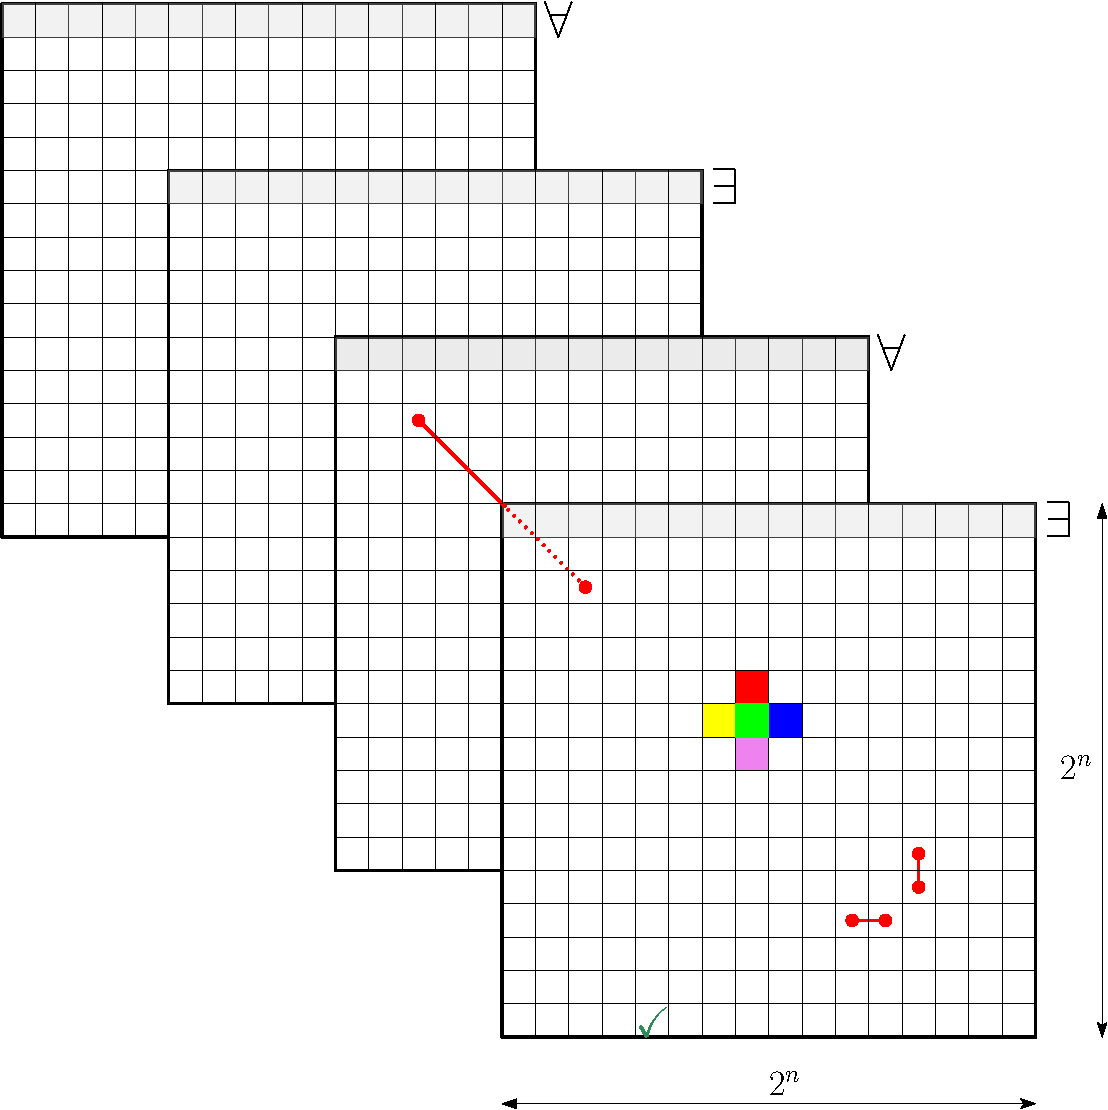
\includegraphics[width=0.9\textwidth]{Chaps/Gandalf17RIVISTA/tiling-crop.pdf}
\caption{The alternating multi-tiling problem (for $n=4$).
The red lines represent the row-adjacency,  column-adjacency, and multi-cell requirements. The green tick denotes the acceptance requirement.
The quantifiers $\forall/\exists$ associated with  the first rows of each tiling mean that the content of these rows has to be universally (resp., existentially) selected, if they belong to an odd (resp., even) tiling.}\label{fig:altmultitil}
\end{figure}

The following complexity result holds (the proof is in Appendix~\ref{proof:theo:ComplexityAlternatingMT}).
\begin{theorem}\label{theo:ComplexityAlternatingMT} The alternating multi-tiling problem is $\LINAEXPTIME\!$-complete
\end{theorem}

The fact that the MC problem for the fragment $\BEbar$ with regular expressions is $\LINAEXPTIME$-hard is an immediate corollary of the following result.

\begin{theorem}\label{theo:MainLowerBoundResult}
One can construct, in time polynomial in the size of $\Instance$, a finite Kripke structure $\Ku_\Instance$ and a $\BEbar$ formula
$\varphi_\Instance$ over the set of proposition letters \[\Prop = D \cup (\{r,c\}\times \{0,1\}) \cup \{\bot,\End\},\]
such that  
$\Ku_\Instance\models \varphi_\Instance$ if and only if $\Instance$ is a \emph{positive} instance of the alternating multi-tiling problem.
\end{theorem}


%\begin{corollary} The model-checking problem for the fragment $\BEbar$ is \LINAEXPTIME-hard.
%\end{corollary}

The rest of this section is devoted to the construction of the Kripke structure $\Ku_\Instance$ and the $\BEbar$ formula
$\varphi_\Instance$ proving Theorem~\ref{theo:MainLowerBoundResult}. Let $\Prop$ be as above. The Kripke structure $\Ku_\Instance$ is given by
$\Ku_\Instance=\KuDef$, where $\States=\Prop$, $\sinit=\End$, $\Lab$ is the identity mapping (we identify
a singleton set $\{p\}$ with $p$), and $\Trans = \{(s,s') \mid s\in \Prop\setminus \{\End\}, s'\in\Prop\}$. Note that the initial state $\End$ has no successors,\footnote{This violates Definition~\ref{def:kripkestructure}, but we define the state $\End$ to have no successors only for technical convenience.}
%and for each state $s$, the set of its predecessors is all $S$. 
and that a trace of $\Ku_\Instance$ can be identified with its induced labeling sequence.

The construction of the $\BEbar$ formula
$\varphi_\Instance$ is based on a suitable encoding of multi-tilings which is described in the following. The symbols
$\{r\}\times   \{0,1\}$ and  $\{c\} \times \{0,1\}$ in $\Prop$
are used to encode the values of two $n$-bits counters numbering the $2^{n}$ rows and  columns, respectively, of a  tiling.

For a multi-tiling $F=\tpl{f_1,\ldots,f_n}$ and for all $i,j\in [0,2^{n}-1]$, the $(i,j)$-{th} \emph{multi-cell} $\tpl{f_1(i,j),\ldots,f_n(i,j)}$ of $F$ is encoded by
the word $C$ of length $3n$ over $\Prop$, called \emph{multi-cell code}, given by
\[C= d_1 \cdots d_n (r, b_1)\cdots(r, b_n)(c,b'_1)\cdots(c, b'_n),\]
where $b_1 \cdots b_n$ and $b'_1\cdots b'_n$ are the binary encodings of the row number $i$ and column number $j$, resp., and for all $\ell\in[1,n]$, $d_\ell= f_\ell(i,j)$ (i.e., the content of the $(i,j)$-th cell of component $f_\ell$).
The \emph{content} of  $C$ is $d_1\cdots d_n$. 
%Note that the structure of a  multi-cell code can be captured by %a regular expression
%$r_{\MC} = D^{n}\cdot (\{r\}\times \{0,1\})^{n}\cdot  %(\{c\}\times \{0,1\})^{n}$.
%
Since $F$ is a multi-tiling,  the following well-formedness requirement must  be satisfied by the encoding $C$: for all $\ell\in [1,n-1]$, $(d_\ell,d_{\ell+1})\in M$. We call such words \emph{well-formed multi-cell codes}.
%The encoding of multi-tilings is as follows.

\begin{definition}[Multi-tiling codes]\label{Def:multiTilingCodes} 
A \emph{multi-tiling code} is a finite word $w$ over $\Prop$  obtained by concatenating well-formed multi-cell codes in such a way  that the following conditions hold:
\begin{itemize}
  \item for all $i,j\in [0,2^{n}-1]$, there is a multi-cell code in $w$  with row number $i$ and column number $j$ \emph{(completeness requirement)};
  \item for all multi-cell codes $C$ and $C'$ occurring in $w$, if $C$ and $C'$ have the same row number and column number, then $C$ and $C'$ have the same content \emph{(uniqueness requirement)};
   \item for all multi-cell codes $C$ and $C'$ in $w$ having the same row number
   (resp., column number), column numbers  (resp., row numbers) $j$ and $j+1$, resp., and contents $d_1\cdots d_n$ and $d'_1\cdots d'_n$, resp., it holds that $(d_\ell,d'_\ell)\in H$ (resp. $(d_\ell,d'_\ell)\in V$) for all $\ell\in [1,n]$ \emph{(row-adjacency requirement)} (resp., \emph{(column-adjacency requirement)});
%  \item for all multi-cell codes $C$ and $C'$ in $w$ having the same row-number, column numbers $j$ and $j+1$, resp., and contents $d_1\ldots d_n$ and $d'_1\ldots d'_n$, resp., it holds that $(d_\ell,d'_\ell)\in H$ for all $\ell\in [1,n]$ \emph{(row-adjacency requirement)};
 %  \item for all multi-cell codes $C$ and $C'$ in $w$ having the same column-number, row numbers $i$ and $i+1$, resp., and contents $d_1\ldots d_n$ and $d'_1\ldots d'_n$, resp., it holds that $(d_\ell,d'_\ell)\in V$ for all $\ell\in [1,n]$ \emph{(column-adjacency requirement)};
  \item there is a multi-cell code in $w$ with row number $2^{n}-1$   whose content is in $D^{n-1}\cdot d_\acc$ for some $d_\acc\in D_\acc$ \emph{(acceptance requirement)}.
\end{itemize}
\end{definition}

%We also need to encode existential and universal quantification on 
Finally, we encode the initial conditions of the components of a multi-tiling.
An \emph{initial cell code} encodes a cell of the first row of a tiling
%
%This leads to the following two Definitions~\ref{Def:InitializationCodes} and~\ref{Def:IMTCodes}, where an \emph{initial cell code} 
and is a word $w$ of length $n+1$ having the form $w =d (c,b_1) \cdots (c,b_n)$, where $d\in D_0$ and $b_1,\ldots,b_n\in \{0,1\}$. We say that $d$ is the \emph{content} of $w$ and the integer in $[0,2^{n}-1]$ encoded by $b_1\cdots b_n$ is the \emph{column number} of $w$. 


\begin{definition}[Multi-initialization codes]\label{Def:InitializationCodes} An \emph{initialization code} is a finite word $w$ over $\Prop$ which is the concatenation of initial cell codes such that:
\begin{itemize}
  \item for all $i \in [0,2^{n}-1]$, there is an initial cell code in $w$  with column number $i$; 
  %\emph{(initial completeness requirement)};
  \item for all initial cell codes $C$ and $C'$ occurring in $w$, if $C$ and $C'$ have the same  column number, then $C$ and $C'$ have the same content.
  %\emph{(initial uniqueness requirement)}.
\end{itemize}
A \emph{multi-initialization code} is a finite word over $\Prop$ having the form $\bot\cdot w_n\cdots \bot \cdot w_1\cdot \End$
such that for all $\ell\in [1,n]$, $w_\ell$ is an initialization code.
\end{definition}

\begin{definition}[Initialized multi-tiling codes]\label{Def:IMTCodes} An \emph{initialized multi-tiling code} is a finite word over $\Prop$ having the form
$\bot \cdot w \cdot \bot\cdot w_n\cdots \bot \cdot w_1\cdot \End$
such that $w$ is a multi-tiling code, $\bot\cdot w_n\cdots \bot \cdot w_1\cdot \End$ is a multi-initialization code, and the following requirement holds:
\begin{itemize}
  \item for each multi-cell code in $w$ having row number $0$, column number $i$, and content $d_1\cdots d_n$, and for all $\ell\in [1,n]$, there is
  an initial cell code in $w_\ell$ having column number $i$ and content $d_\ell$  \emph{(initialization coherence requirement)}.
\end{itemize}
\end{definition}

Before proving Theorem~\ref{theo:MainLowerBoundResult},
we sketch the idea for the construction of the $\B\Ebar$ formula $\varphi_\Instance$ which guarantees that $\Ku_\Instance\models \varphi_\Instance$ if and only if $\Instance$ is a positive instance of the alternating multi-tiling problem. 

We preliminarily  observe that  since the initial state of $\Ku_\Instance$ has no successors, the only initial trace of $\Ku_\Instance$ is the trace $end$ having length 1. To guess a trace corresponding to an initialized multi-tiling code, $\Ku_\Instance$ is unraveled backward starting from $end$, exploiting the modality $\Ebar$. The structure of the formula $\varphi_\Instance$ is 
\[
\varphi_\Instance= \hsEtu(\varphi_1 \rightarrow \hsEt(\varphi_2\wedge(\ldots (\hsEtu(\varphi_{n-1} \rightarrow \hsEt(\varphi_n\wedge \hsEt \varphi_\IMT)))\ldots))).
\]
It features $n+1$ unravelling steps starting from the initial trace $end$. The first $n$ steps are used to guess a sequence of $n$ initialization codes. Intuitively, each formula $\varphi_i$ is used to constrain 
the $i$-th unravelling to be an initialization code, in such a way that at depth $n$ in the formula a multi-initialization code is under evaluation. 
The last unravelling step (the innermost in the formula) is used to guess the multi-tiling code. The innermost formula $\varphi_\IMT$ is evaluated over a trace corresponding to an initialized multi-tiling code, and checks its structure: 
multi-cell codes are \lq\lq captured\rq\rq{} by regular expressions (encoding in particular their row and column numbers and contents).
The completeness, uniqueness, row- and column-adjacency requirements for the multi-tiling of Definition~\ref{Def:multiTilingCodes} are enforced by the combined use of the $\hsEtu$ modality and regular expressions.

The intuition of such a technique is graphically depicted in Figure~\ref{fig:multicod}, where $w$ is a multi-tiling code.
Since the problem is to check constraints between pairs of multi-cell codes occurring in arbitrary positions of $w$, we use the following trick. A copy of two multi-cell codes $C$ and $C'$ (see Figure~\ref{fig:multicod}) are generated next to each other, as backward extensions of the initialized multi-tiling code, by means of modality $\hsEtu$. We then check that both $C$ and $C'$ occur in (arbitrary positions of) $w$, and, if this is the case, the required constraint is checked against the generated copies $C$ and $C'$, taking advantage of their adjacency. 
%
%In order to check the constraints between two pairs of multicell occurring in i
%by means of $\hsEtu$, one or two multi-cell codes are generated \lq\lq separately\rq\rq; then, if they appear in the considered multi-tiling code, the aforementioned constraints are verified by means of auxiliary formulas, consisting of suitable regular expressions. See Figure~\ref{fig:multicod}.
\begin{figure}[tp]
    \centering
    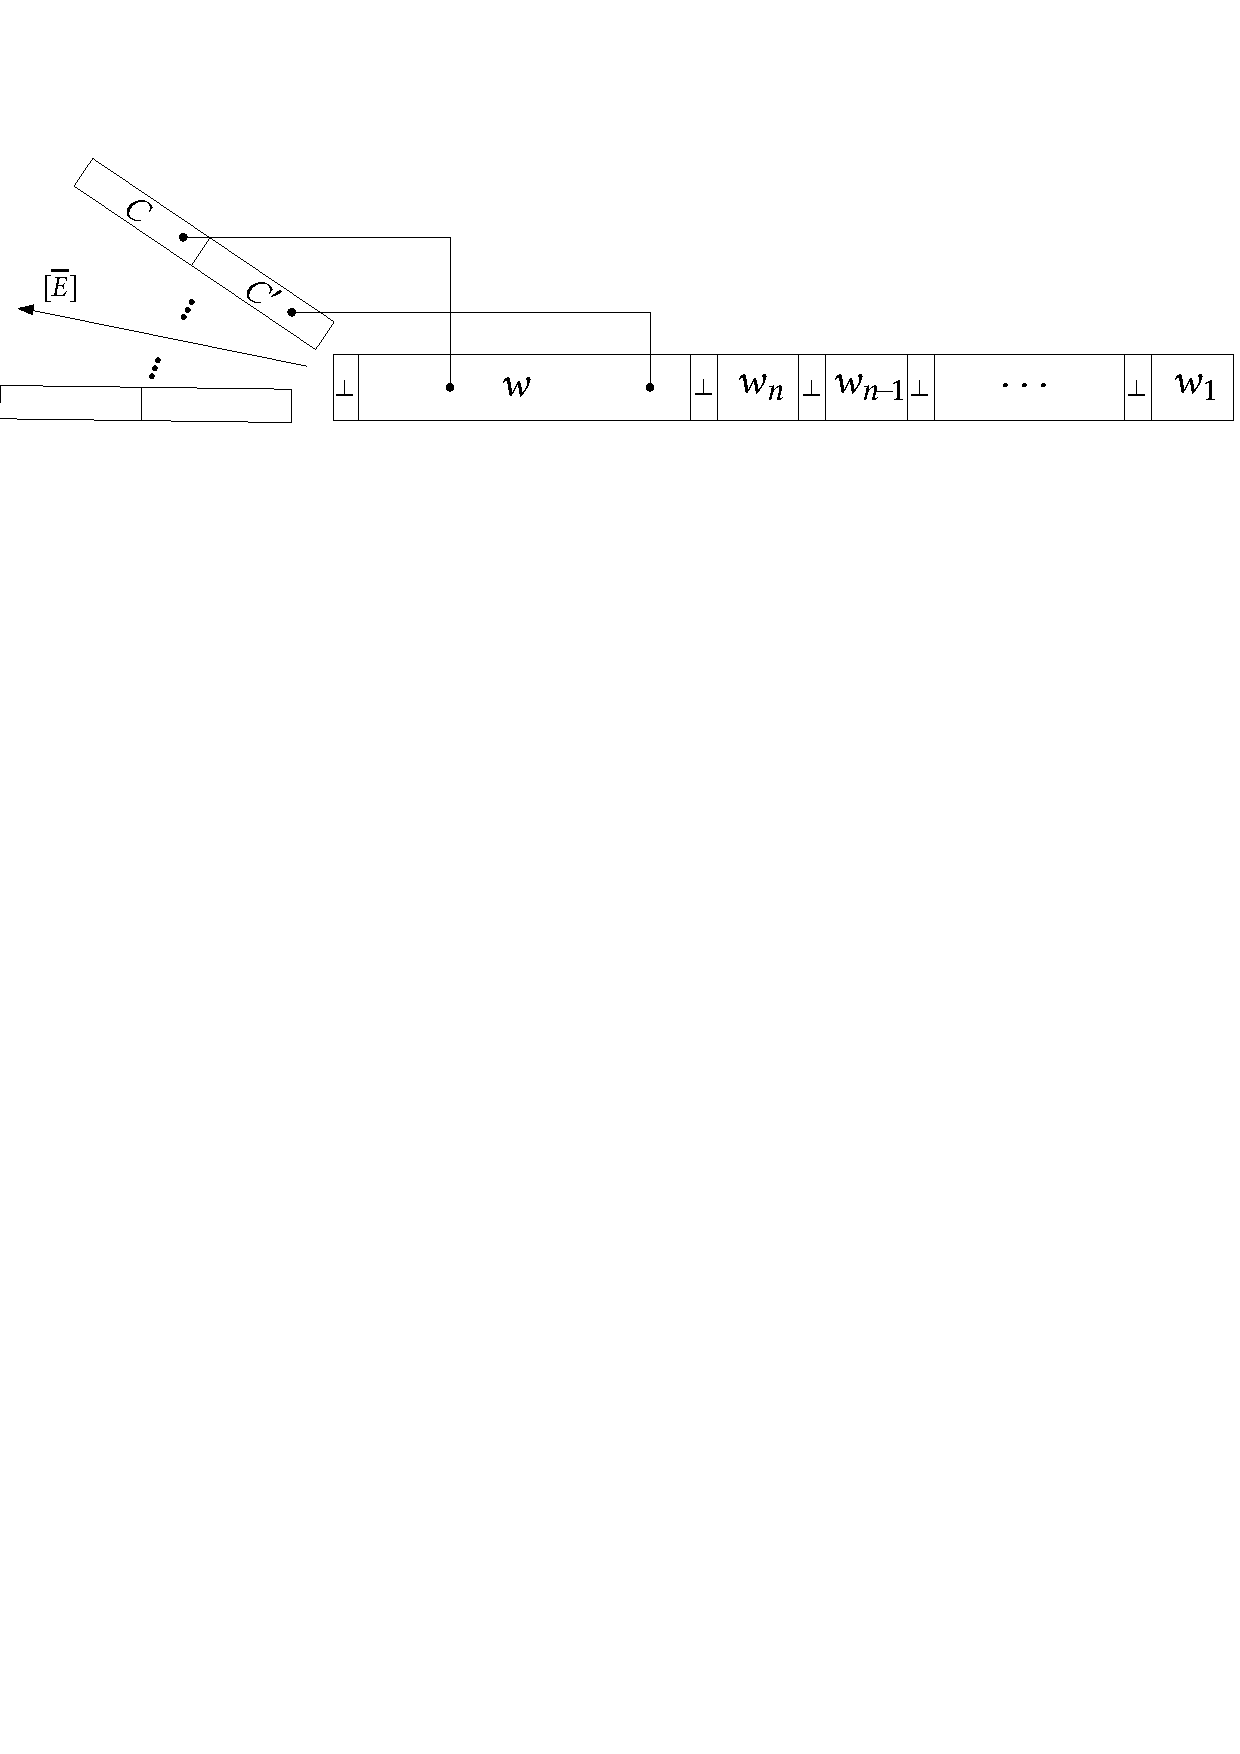
\includegraphics[width=\textwidth]{Chaps/Gandalf17RIVISTA/multicod.pdf}
    \caption{Checking constraints between pairs of multi-cell codes $C$ and $C'$ in an initialized multi-tiling code.}
    \label{fig:multicod}
\end{figure}
%
The initialization coherence requirement of Definition~\ref{Def:IMTCodes} is guaranteed in an analogous way, by comparing initial cell codes and multi-cell codes.

Note that the first $n-1$ occurrences of alternations between universal and existential modalities  $\hsEtu$ and $\hsEt$ correspond to the alternations of universal and existential quantifications in the definition of alternating multi-tiling problem. 

The correctness of the construction of $\varphi_\Instance$ is stated by the next proposition.
%
\begin{proposition}\label{prop:FormulasForMultiTilingCodes}  One can build, in  time polynomial in the size of $\Instance$,
$n+1$ $\BEbar$ formulas $\varphi_\IMT,\varphi_1,\ldots,\varphi_n$ with $\AltN(\varphi_\IMT)=\AltN(\varphi_1) =\ldots =\AltN(\varphi_n)= 0$, fulfilling the following conditions:
\begin{itemize}
  \item for all finite words $\rho$ over $\Prop$ having the form $\rho =\rho' \cdot \bot \cdot w_n  \cdots  \bot \cdot w_1\cdot \End$ such that $\rho'\neq \varepsilon$ and
  $\bot \cdot w_n  \cdots  \bot \cdot w_1\cdot \End$ is a multi-initialization code, it holds that $\Ku_\Instance,\rho\models\varphi_\IMT$ if and only if
  $\rho$ is an initialized multi-tiling code;
  \item for all $\ell\in [1,n]$ and words $\rho$ having the form $\rho=\rho'\cdot \bot \cdot w_{\ell-1} \cdots \bot \cdot w_1\cdot \End$ such that
 $\rho'\neq \varepsilon$ and $w_j\in (\Prop\setminus \{\bot\})^{*}$ for all $j\in [1,\ell-1]$, it holds that $\Ku_\Instance,\rho\models\varphi_\ell$ if and only if
$\rho'$ has the form  $\rho'=\bot\cdot w_\ell$, where $w_\ell$ is an initialization code.
\end{itemize}
\end{proposition}
\begin{proof}
Since each state of the Kripke structure $\Ku_\Instance$ is labeled by exactly one proposition letter of $\Prop$, in the proof we exploit the standard regular expressions, where atomic expressions are single letters of $\Prop$. Evidently, a standard regular expression can be converted into a proposition-based one, where each $p\in\Prop$ is replaced by the formula $p\wedge \bigwedge_{p'\in\Prop\setminus \{p\}}\neg p'$. 

Let us focus on the construction of the $\BEbar$ formula $\varphi_\IMT$ (as $\varphi_1,\ldots,\varphi_n$ are simpler).
First, we define a $\BEbar$ formula $\varphi_\MT$ ensuring the following property:
\begin{itemize}
  \item for all finite words $\rho$ over $\Prop$ having the form  $\rho =\rho' \cdot \bot \cdot w_n \cdots \bot \cdot w_1\cdot \End$ such that $\rho'\neq \varepsilon$ and
  $\bot \cdot w_n \cdots \bot \cdot w_1\cdot \End$ is a multi-initialization code, it holds $\Ku_\Instance,\rho\models\varphi_\MT$ if and only if
  $\rho'=\bot\cdot w$ for some multi-tiling code $w$.
\end{itemize}

In order to build $\varphi_\MT$, we need some auxiliary formulas and regular expressions.
%
\begin{itemize}
\item A regular expression $r_{\MC} = D^{n}\cdot (\{r\}\times \{0,1\})^{n}\cdot  (\{c\}\times \{0,1\})^{n}$ capturing the multi-cell codes.
%\[
%r_{\MC} = D^{n}\cdot (\{r\}\times \{0,1\})^{n}\cdot  (\{c\}\times \{0,1\})^{n}
%\]
\item    A $\B$ formula $\psi_{\Complete}$ requiring that for each word $C\cdot   \bot \cdot C_1 \cdots C_N\cdot \bot$ such that
  $C, C_1,\ldots,C_N$ are multi-cell codes,
   there is $i\in [1,N]$ such that $C$ and $C_i$ have the same row number and column number.
\begin{multline*}
    \psi_{\Complete} \! = \! \hsB \Bigl((r_{\MC}\cdot \bot \cdot (r_{\MC})^{+}) \wedge \!\!\!
    \bigwedge_{i\in [1,n]}\bigvee_{b\in \{0,1\}}\!\!\!\!\!(\Prop^{n+i-1}\cdot (r,b) \cdot \Prop^{+}\cdot  (r,b)\cdot \Prop^{2n-i}) \wedge
    \\
     \bigwedge_{i\in [1,n]}\bigvee_{b\in \{0,1\}}(\Prop^{2n+i-1}\cdot (c,b) \cdot \Prop^{+}\cdot   (c,b)\cdot \Prop^{n-i})\Bigr)
\end{multline*}

 \item A propositional formula $\psi_=$ requiring that for each word having as a proper prefix $C\cdot C'$ such that $C$ and $C'$ are multi-cell codes,
 $C$ and $C'$ have the same row number and column number.
\begin{multline*}
    \psi_{=}  =  \bigwedge_{i\in [1,n]}\bigvee_{b\in \{0,1\}}(\Prop^{n+i-1}\cdot (r,b) \cdot \Prop^{3n-1}\cdot (r,b)\cdot \Prop^{+})\wedge
    \\
    \bigwedge_{i\in [1,n]}\bigvee_{b\in \{0,1\}}(\Prop^{2n+i-1}\cdot (c,b) \cdot \Prop^{3n-1}\cdot (c,b)\cdot \Prop^{+})
\end{multline*}
 \item A propositional formula $\psi_{\RInc}$ (resp., $\psi_{\CInc}$) requiring that for each word having as a proper prefix $C\cdot C'$ such that $C$ and $C'$ are multi-cell codes,
 $C$ and $C'$ have the same column number (resp., the same row number), and there is $h\in [0,2^{n}-2]$ such that $C$ and $C'$ have row numbers (resp., column numbers) $h$ and $h+1$, resp.. We consider the formula $\psi_{\RInc}$ (the definition of $\psi_{\CInc}$ is similar).
\begin{multline*}
    \psi_{\RInc}  = \bigwedge_{i\in [1,n]}\bigvee_{b\in \{0,1\}}(\Prop^{2n+i-1}\cdot (c,b) \cdot \Prop^{3n-1}\cdot (c,b)\cdot \Prop^{+})\wedge
    \\
    \bigvee_{i\in [1,n]}\Bigl(\bigwedge_{j\in [1,i-1]}(\Prop^{n+j-1}\cdot (r,1) \cdot \Prop^{3n-1}\cdot (r,0)\cdot \Prop^{+})\wedge
    \\
     (\Prop^{n+i-1}\cdot (r,0) \cdot \Prop^{3n-1}\cdot (r,1)\cdot \Prop^{+})\wedge
    \\
    \bigwedge_{j\in [i+1,n]} \bigvee_{b\in \{0,1\}}(\Prop^{n+j-1}\cdot (r,b) \cdot \Prop^{3n-1}\cdot (r,b)\cdot \Prop^{+})\Bigr)
\end{multline*}
%
 \item A $\B$ formula $\psi_{\Double}$ requiring that for each word $C\cdot C'\cdot \bot \cdot C_1 \cdots C_N\cdot \bot$ such that
  $C,C',C_1,\ldots,C_N$ are multi-cell codes, there are $i,j\in [1,N]$ such that $C=C_i$ and $C'=C_j$;
  $\psi_{\Double} = \theta \wedge \theta'$, where $\theta$ (resp., $\theta'$) requires that
  there is $i\in [1,N]$ such that $C_i=C$ (resp., $C_i=C'$). We consider $\theta'$ (the definition of $\theta$ is similar).
\begin{multline*}
    \theta'  = \hsB \Bigl((r_{\MC}\cdot r_{\MC} \cdot \bot \cdot (r_{\MC})^{+})\wedge
    \bigwedge_{i\in [1,n]}\bigvee_{d\in D}(\Prop^{3n+i-1}\cdot d \cdot \Prop^{+}\cdot  d\cdot \Prop^{3n-i})\wedge
    \\
    \bigwedge_{i\in [1,n]}\bigvee_{b\in \{0,1\}}(\Prop^{4n+i-1}\cdot (r,b) \cdot \Prop^{+}\cdot  (r,b)\cdot \Prop^{2n-i})\wedge
    \\
    \bigwedge_{i\in [1,n]}\bigvee_{b\in \{0,1\}}(\Prop^{5n+i-1}\cdot (c,b) \cdot \Prop^{+}\cdot   (c,b)\cdot \Prop^{n-i})\Bigr)
\end{multline*}
%
  \item A $\B$ formula $\psi_{\NU}$ requiring that for each word $C\cdot C'\cdot \bot \cdot C_1 \cdots C_N\cdot \bot$ such that
  $C,C',C_1,\ldots,C_N$ are multi-cell codes, the next properties hold:
  \begin{itemize}
    \item $C$ and $C'$ have the same row and column numbers, but different content;
    \item there are $i,j\in [1,N]$ such that $C=C_i$ and $C'=C_j$.
  \end{itemize}
  The construction of $\psi_{\NU}$ is based on the formulas $\psi_{\Double}$ and $\psi_=$:
\begin{multline*}
    \psi_{\NU}  = \psi_{\Double} \wedge  \psi_= \wedge \bigvee_{i\in [1,n]}\bigvee_{d,d'\in D:d\neq d'}(\Prop^{i-1}\cdot d \cdot \Prop^{3n-1}\cdot d'\cdot \Prop^{+}).
\end{multline*}
%
\item A $\B$ formula $\psi_{\Row}$ (resp., $\psi_{\Column}$) requiring that for each word $C\cdot C'\cdots C_1 \cdots C_N\cdot \bot$ such that
  $C,C',C_1,\ldots,C_N$ are multi-cell codes, the next condition holds.
  \begin{itemize}
    \item Let us denote by $d_1\cdots d_n$ the content of $C$ and by $d'_1\cdots d'_n$ the content of $C'$. Whenever $(1)$~there are $i,j\in [1,N]$ such that $C=C_i$ and $C'=C_j$, and $(2)$~$C$ and $C'$ have the same row number and column numbers $h$ and $h+1$, resp. (resp., $C$ and $C'$ have the same column number and row numbers $h$ and $h+1$, resp.) for some $h\in [0,2^{n}-2]$,
         then it holds that $(d_\ell,d'_\ell)\in H$ (resp., $(d_\ell,d'_\ell)\in V$), for all
        $\ell\in [1,N]$.
  \end{itemize}
We focus on $\psi_{\Row}$ (the definition of $\psi_{\Column}$ is similar): 
%whose construction is based   on the formulas %$\psi_{\Double}$ and $\psi_{\CInc}$:
\begin{multline*}
    \psi_{\Row}  = (\psi_{\Double} \wedge  \psi_{\CInc})  \longrightarrow  \bigwedge_{i\in [1,n]}\bigvee_{(d,d')\in H}(\Prop^{i-1}\cdot d \cdot \Prop^{3n-1}\cdot d'\cdot \Prop^{+}).
\end{multline*}
\end{itemize}

Finally, the $\BEbar$ formula  $\varphi_\MT$ is defined as follows:
\begin{multline*}
\neg (\Prop^{*}\cdot \bot \cdot \Prop^{*})^{n+2} \wedge
 \hsB \Bigl(\underbrace{(\bot\cdot (r_{\MC})^{+} \cdot \bot)\wedge\neg \bigvee_{(d,d')\in D^{2}\setminus M}(\Prop^{+}\cdot d\cdot d'\cdot \Prop^{+})}_{\text{Concatenation of well-formed multi-cell codes}}\wedge
\\
 \underbrace{\hsEtu((r_{\MC}\cdot \bot\cdot (r_{\MC})^{+} \cdot \bot) \longrightarrow \psi_\Complete)}_{\text{Completeness requirement of Definition \ref{Def:multiTilingCodes}}}\wedge
 \\
\underbrace{\hsEtu((r_{\MC}\cdot r_{\MC}\cdot \bot\cdot (r_{\MC})^{+} \cdot \bot) \longrightarrow \neg\psi_{\NU})}_{\text{Uniqueness requirement of Definition \ref{Def:multiTilingCodes}}}\wedge
\\
\underbrace{\hsEtu((r_{\MC}\cdot r_{\MC}\cdot \bot\cdot (r_{\MC})^{+} \cdot \bot) \longrightarrow (\psi_{\Row}\wedge \psi_{\Column}))}_{\text{Row-adjacency and column-adjacency requirements of Definition \ref{Def:multiTilingCodes}}}\wedge
\\
\underbrace{\bigvee_{d_\acc\in D_\acc}(\Prop^{+}\cdot d_\acc \cdot (r,1)^{n}\cdot \Prop^{+}) }_{\text{Acceptance requirement of Definition \ref{Def:multiTilingCodes}}}\Bigr).
\end{multline*}

The $\BEbar$ formula $\varphi_\IMT$ is given by
%\[
$\varphi_\MT\wedge \varphi_\Coh$,
%\]
where $\varphi_\Coh$ ensures the initialization coherence requirement of Definition~\ref{Def:IMTCodes}. In order to define
$\varphi_\Coh$, we need some auxiliary formulas and regular expressions.
\begin{itemize}
\item A regular expression $r_{\IC} = D_0 \cdot   (\{c\}\times \{0,1\})^{n}$ capturing the  initial cell codes.
%\[
%r_{\IC} = D_0 \cdot   (\{c\}\times \{0,1\})^{n}.
%\]
\item    A $\B$ formula $\psi_{\Single}$ requiring that for each word $C\cdot   \bot \cdot C_1 \cdots C_N\cdot \bot$ such that
  $C, C_1,\ldots,C_N$ are multi-cell codes,
   there is $i\in [1,N]$ such that $C=C_i$ and  the row number of $C$ is $0$. The definition of $\psi_\Single$ is similar to $\psi_\Double$.
 \item A $\B$ formula $\psi_{\Coh}$ requiring that for each word $C\cdot   \bot \cdot C_1 \cdots C_N\cdot \bot \cdot w_n \cdots \bot \cdot w_1 \cdot \End$ such that   $C, C_1,\ldots,C_N$ are multi-cell codes and $\bot \cdot w_n \cdots \bot \cdot w_1 \cdot \End$ is a multi-initialization code, the following constraint holds:
     if   there is $i\in [1,N]$ such that $C=C_i$, the row number of $C$ is $0$ and the content of $C$ is $d_1\cdots d_n$, then for all $\ell\in [1,n]$, there exists an initial code in $w_\ell$ having the same column number as $C$ and content $d_\ell$.
\[
\psi_\Coh  =   \bigl( \hsB( [(\Prop\setminus \{\bot\})^{+} \cdot \bot \cdot (\Prop\setminus \{\bot\})^{+} \cdot \bot] \wedge \psi_\Single)  \bigr) \longrightarrow \displaystyle{\bigwedge_{\ell\in [1,n]}\psi_\ell};
\]

\begin{multline*}
\psi_\ell =   \hsB\Bigl(\bigl[(\Prop\setminus \{\bot\})^{+}\cdot (\bot \cdot (\Prop\setminus \{\bot\})^{+})^{n-\ell+1}\cdot \bot \cdot r_\IC^{+}  \bigr] \wedge
\\
\bigwedge_{i\in [1,n]}\bigvee_{b\in \{0,1\}}(\Prop^{2n+i-1}\cdot (c,b) \cdot \Prop^{+}\cdot (c,b)\cdot \Prop^{n-i})\wedge
\\
 \bigvee_{d\in D}(\Prop^{\ell-1}\cdot d \cdot \Prop^{+}\cdot d\cdot \Prop^{n})\Bigr).
\end{multline*}
\end{itemize}
The  $\BEbar$ formula $\varphi_\Coh$ is then 
%\[
$\varphi_\Coh = \hsEtu\bigl([r_\MC\cdot (\bot \cdot (\Prop\setminus \{\bot\})^{+})^{n+1}  ]  \rightarrow \psi_\Coh\bigr)$.
%\]

This concludes the proof of Proposition~\ref{prop:FormulasForMultiTilingCodes}.
\end{proof}

Recall that
%\[
$\varphi_\Instance\!=\! \hsEtu(\varphi_1 \rightarrow \hsEt(\varphi_2\wedge(\ldots (\hsEtu(\varphi_{n-1} \rightarrow \hsEt(\varphi_n\wedge \hsEt \varphi_\IMT)))\ldots))),$
%\]
where $\varphi_\IMT,\varphi_1,\ldots,\varphi_n$ are the formulas defined in Proposition~\ref{prop:FormulasForMultiTilingCodes}.
Since the initial state of $\Ku_\Instance$ has no successors and the only initial trace has length 1 and corresponds to the proposition letter $\End$, by Definitions~\ref{Def:multiTilingCodes}--\ref{Def:IMTCodes}, we have that
$\Ku_\Instance\models \varphi_\Instance$ if and only if $\Instance$ is a positive instance of the alternating multi-tiling problem, proving  Theorem~\ref{theo:MainLowerBoundResult}. This result, combined with Theorem~\ref{Theorem:UpperBoundAAbrBBarEbar}, implies the following.

\begin{corollary}
The MC problem for $\AAbarBBbarEbar$ (and $\AAbarEBbarEbar$) formulas extended with regular expressions over finite Kripke structures is \mbox{$\LINAEXPTIME$-complete}.
\end{corollary}